L’évaluation des performances se décomposent des différents éléments suivants, et qui sont présentés dans le diagramme de la figure \ref{fig:metho_eval}: 
\begin{itemize}
    \item Tout d'abord, les indicateurs de performances.
    \begin{itemize}
        \item Les performances matérielles durant l'inférence seront évaluées grâce aux indicateurs fournies par les utilitaires 'Tegrastats' de NVIDIA, 'free' et 'iotop'. Ces utilitaires sont brièvement décrit dans le tableau \ref{table:table_sol_logiciel}.
        \item Les performances de la segmentation seront évaluées avec les indicateurs classiques\footnote{\url{https://ilmonteux.github.io/2019/05/10/segmentation-metrics.html}}: "IoU" ("Intersection Over Union", ou "Jaccard") et le "Z-Score" (ou "Dice").
    \end{itemize}
    \item Ensuite, différentes résolutions d'images et de vidéos seront utilisées pour déterminer lesquelles sont supportées par le modèle évalué. 
    \item Les images et vidéos qui sont à notre disposition pour être évaluée proviennent de différentes sources de données. Le jeu d'images de DeepScene est celui qui semble le plus approprié car il a été conçu pour détecter les chemins dans la forêt. De plus il existe une version du modèle qui a été entrainé avec ce jeu. Comme il possède un jeu d'images vérité terrain ("ground truth" GT), il sera bien utile pour évaluer la segmentation prédite et un gain de temps non négligeable dans le cadre d'un essai. Le jeu d'images de CityScape est très complet pour les scènes urbaines, mais comme il est moins spécialisé dans la détection de chemins ou de piste, son utilisation ne sera pas priorisé. Il contient toutefois des images vérité terrain de routes, ce qui est avantageux dans notre contexte et le favorise  par rapport au deux derniers que nous avons à notre disposition. En effet le jeu d'images et de vidéos de l'Association des piétons et cyclistes du pont Jacques-Cartier, et celui que j'ai monté, sont des jeux intéressants pour tester les résultats de la segmentation avec des images ou des vidéos qui viennent du site d'études, ou similaire, que celui de chemins forestiers. De plus ces images et vidéos sont loin des conditions parfaites (luminosité, qualité du sol, angle de vue, etc).
    \item Enfin plusieurs modèles ont été sélectionnés comme candidats intéressants pour l'évluation. Le premier modèle qui sera évalué sera celui de SegNet18 entrainé avec le jeu de données "DeepSCene", et fourni par NVIDIA. Le second de la liste, et qui est aussi déjà founi par NVIDIA, est celui de SegNet18 entrainé avec le jeu de donnée "CityScape". Les deux autres architectures, ResNet101 \& DeepScene et DeepLabV3 \& Deepscene, ne sont pas disponibles et devront être préparées et entrainées, mais elles sont attrayantes du point de vue de leur réputation et potentiel, et vouloir les adapter au contexte de l'essai semble logique. Une dernière boîte vide est disponible, afin de laisser une porte ouverte à une potentielle opportunité d'entrainer un modèle tout à fait personnalisé, comme par exemple une adapation de l'architecture de DeepLabV3 avec le jeu de données de l'Association des piétons et cyclistes du pont Jacques-Cartier.
\end{itemize} 
\label{metho_eval}
\begin{figure}[H]
    \centering
    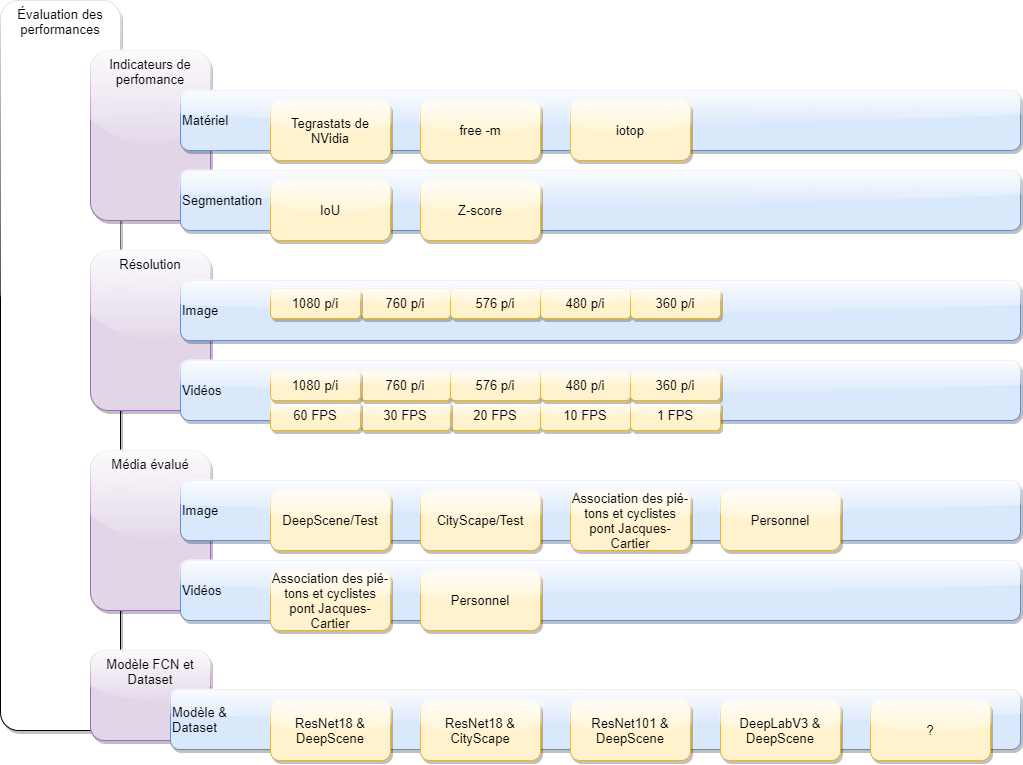
\includegraphics[width=1.0\textwidth]{metho_eval_perf_round_glass_shadow2}
    \caption{Éléments pour l'évaluation des performances}
    \label{fig:metho_eval}
\end{figure}
\subsubsection{Stratégie de test de l'inférence} \label{section:strategie_test_inference}
\par L'objectif principal de l'essai est de déterminer la capacité et les limites du nano ordinateur d'inférer en temps réel des modèles de réseau de neurones à convolution entier pour la segmentation sémantique de vidéos. La stratégie qui sera appliquée sera de tester avec divers modèles et divers niveaux de qualité vidéos, en espérant trouver le compromis qui répond le mieux à cet objectif.
\begin{enumerate}
   \item \label{metho:testbaseinférence} Afin de s'assurer du bon fonctionnement du nano ordinateur et d'avoir des résultats de référence propre à notre environnement, l'inférence sera testée avec des modèles existants et pré entrainés pour la segmentation sémantique, avec les images et les vidéos provenant des références, et dont les caractéristiques et les résultats sont disponibles. 
   \item \label{metho:testbaseinférencesite} En espérant que les tests de l'étape \#\ref{metho:testbaseinférence} précédente donnent les résultats documentés dans les articles de références, ils seront repris avec les mêmes modèles, mais avec les images et les vidéos du site d'étude possédant la meilleure qualité acquise (1080p/i, 30\acrshort{fps}). Les données sources (images et vidéos) devront subir certains prétraitements à ce effet, afin de répondre aux requis des modèles.
   \item \label{metho:testdevinférencesite} Selon les résultats de l'étape \#\ref{metho:testbaseinférencesite}, les tests se concentreront sur l'inférence avec des vidéos, en réduisant progressivement la résolution (760p/i, 576p/i, 480p/i, 360p/i) et le nombre d'images par seconde (20\acrshort{fps}, 10FSP, 1\acrshort{fps}).
   \item Les étapes intermédiaires de l'étape \#\ref{metho:testdevinférencesite} précédente seront de 1) valider les résultats de l'inférence avec des images avant de tester avec les vidéos, et 2) évaluer si les modèles de réseaux de neurones à convolution entiers doivent et/ou peuvent être adaptés facilement, en tenant compte de l'échéancier de l'essai, et ce afin de répondre à l'objectif principal.
\end{enumerate}
\subsubsection{Stratégie de collecte des indicateurs de performance matériel}
\par La méthodologie de la collecte des indicateurs est la suivante\footnote{\url{https://vince7lf.github.io/2020/05/26/metrics.html}}: 
\begin{itemize}    
    \item La collecte est démarrée après un démarrage frais, manuellement, via un script shell, qui exécute chaque utilitaire, et attend l'interruption du test. 
    \item Chaque utilitaire qui est utilisé pour collecter les mesures, possède son propre fichier.
    \item La date et l'heure de chaque indicateur collecté sont précisées.
    \item Afin de faciliter la documentation et l'analyse du test, des points d'intérêt sont ajoutés dans un fichier séparé pour marquer un moment particulier du test, avec la date, l'heure et un libellé. Ce point d'intérêt est fait grâce à une commande "shell" qui vient ajouter une trace dans ce fichier.
    \item Chaque indicateur est collecté toutes les secondes.  
    \item Une fois le test complété, la collecte est arrêté manuellement. 
    \item Chaque fichier est ensuite transformé en fichier CSV, via des commandes shell.
    \item À partir des fichiers CSV un script Python génère les graphiques automatiquement. 
\end{itemize}
\par Chaque indicateur est une colonne du fichier CSV. Il existe le même nombre d'indicateurs à tout moment. La date et l'heure sont un champ. 
\par Avant tout début de tests, la collecte est démarrée sans activité autre que la collecte des indicateurs. Cela permet de prendre une base de référence sans aucune charge.
\par Ensuite les tests débutent. 
\par Les indicateurs collectés permettent de créer des graphiques qui montrent la progression de chacun.
\par Les performances matérielles du Jetson Nano sont évaluées grâce à différents utilitaires : "tegrastats" fournis par NVIDIA, "free" et "iotop".
\par Les performances de la segmentation sont évaluées grâce au\acrshort{iou}et au z-score pour la classe du chemin / route. Une fonction Python est utilisée. Les fonctions\acrshort{iou}et le z-score utilisent l'image prédite (généré par le modèle FCN) et l'image vérité terrain ("ground truth"). Les images originales sont donc présélectionnées selon leur intérêt et l'image vérité terrain ("ground truth") créée. L'image prédite et vérité terrain ("ground truth") doivent utiliser la même palette de couleurs et doivent être de la même résolution. Pour les images qui ne possèdent pas d'image vérité terrain ("ground truth"), cell-ci est créée à la main avec l'éditeur "Gimp". Comme la résolution de la segmentation de l'image prédite par le modèle de NVIDIA est très faible ("carrée"), l'image vérité terrain ("ground truth") ne sera pas précise au pixel prêt. Le besoin est d'évaluer et non d'entrainer, l'importance de la précision de la classification est moindre dans ce cas. 